\section{Exercice 2 : Conversion d'une image couleur en niveau de gris}
\begin{enumerate}
  \item
        \q{Convertir l'image en noveau de gris avec la fonction }
        \il{convert}\q{ et faire afficher le résultat.}

        \begin{dinglist}{111}
          \item
          Dans le dossier \il{ressources}, je crée un fichier \il{helpers.py}
          dans lequel je crée la fonction \il{plotImage} qui me servira aussi
          pour les exerices suivants.\\
          Elle permet de rajouter plusieurs images sur le même \il{plot}.
          Elle ne lance le rendu de toutes les images que si le paramètre
          \il{show} est passé à \il{True}.

          \newpage

          \codeFromFile{section-02/q1-1.py}

          \item
          Ensuite, je convertis l'image et j'affiche le avant-après.
          \codeFromFile{section-02/q1-2.py}
          \begin{center}
            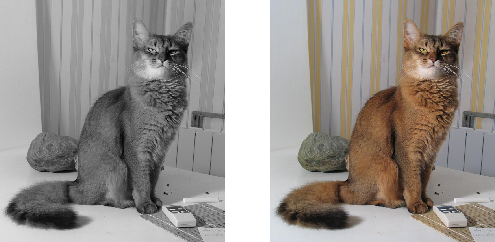
\includegraphics[scale=0.5]{section-02/q1-3.png}
          \end{center}
        \end{dinglist}
  \item
        \q{Ecrire une fonction qui retroune un tableau de niveau de gris d'une image.}
        \codeFromFile{section-02/q2.py}
  \item
        \q{Créer une image depuis le tableau précédent.}
        \newpage
        \codeFromFile{section-02/q3.py}
        Il suffit maintenant d'éxecuter \il{greyScaleImg = arrayToImage(geryScale(img))}
        pour avoir le tableau demandé.
  \item
        \q{Enregistrer cette image.}
        \codeFromFile{section-02/q4.py}
\end{enumerate}
